This chapter outlines future work to be performed as part of the project, split into different areas of focus. Specific research questions (RQs) are identified along with associated sub-research questions (SRQs). Later areas of research do not yet have specifically defined research questions, which will be determined nearer to the time.

\section{Reverse Engineering Output}\label{future-reveng}

Complete integration of reverse engineering work within D-UEA-ST framework with respect to re-projection of UML within UMLet, specifically integrate relationships into the projection. Also investigate the possibility of using time-based evolution with reverse engineering. Look further into the gaps found in poor-performing reverse engineering software.

\textbf{RQ. Is there any advantage to providing a sequential series of reverse engineering ``snapshots'' linked to the development of the software over time (reconstructed at points from source code repositories)?}

\textbf{RQ. For ``missing information'' in poor reverse engineering, is this the same common information between different reverse engineering applications?}

\textbf{SRQ. Can we build a more complete structural picture from multiple poor pictures e.g. can we combine output from more than one tool and form a more complete output?}

\section{Co-Commit Information}\label{future-cocomm}

Refine co-commit toolchain to replace IBDOOS inclusion for efficiency. Test this technique with repositories other than git. Analyse the output generated from Co-Comm data to quantify its usefulness as applied to traceability reconstruction.

\textbf{RQ. Does co-commit data show ``sensible'' (and useful) relationships?}

\textbf{RQ. What is the correlation between relationships identified through co-commit information and those through reverse engineering?}

\textbf{SRQ. Can relationships identified through reverse engineering be augmented through co-commit relationships?}

\section{Clustering of Related Components}

Continue to investigate clustering techniques and their application to the data generated from different sources. Specifically work to refine the EM model and find appropriate settings to cluster software components, ideally at different levels such as sub-clusters.

\textbf{RQ. What clustering techniques are most suited to software components?}

\textbf{RQ. Can clustering provide a more useful picture of relationships between components than purely similarity/dissimilarity numbers?}

\textbf{RQ. Can different data sources be combined to better inform clustering either pre-cluster (combined similarity matrices) or post-cluster (average of cluster memberships)?}

\textbf{RQ. Can clustering be used to determine parts of software architectural styles such as model-view-controller?}

\section{Other Sources of Information}

Investigate other potential sources of information and methods to integrate them into existing toolchains.

\subsection{Requirements Documentation}

In association with an MSc project in 2013/14 perform textual analysis of requirements documentation (using techniques such as natural language processing). Link documentation to components within software (possibly performing transformation to allow source-code to be textually examined).

\subsection{Technical Documentation and Code Comments}

Investigate integration of more specific technical documentation (API documentation etc), most likely in a similar method to requirement documentation.

Work to integrate source code comments (such as Javadoc but also more generalised comments) into visualisation and/or description of software at a model level, and as potential indicators to relationship between requirements and implementation.

\subsection{Runtime Relationship/Dependency Information}

Investigate the possibility of incorporating run-time information such as call traces into augmenting relationship information.

\textbf{RQ. Is effective runtime analysis possible in larger applications?}

\textbf{SRQ. Can collection of runtime information be automated in terms of collection of state types?}

\textbf{RQ. Does runtime relationship analysis show different relationships to other information sources such as reverse engineering?}

\textbf{SRQ. What is the overlap between runtime and other information sources relationships?}

\textbf{RQ. Can runtime information be usefully integrated to provide additional information?}

\subsection{Existing Software Library}

Investigate the possibility of building a library of existing software for which certain information is known, for example for which previous manual analysis has been performed. This library would consist of not just source code and resultant analysis but also a set of abstracted structural representations at different levels which may be used for pattern matching.

\section{Reasoning Component}

Work towards the development of a reasoning component to augment decision making in terms of detection of components and links between levels of information. This will be a semi-manual process involving a weighted set of data sources being provided (possibly analysed for accuracy through a visualisation application). All types of data input will be supported e.g. reverse engineering, co-commit data, clustering output etc. The infrastructure will be extensible allowing for inclusion of more data sources as they become available. The reasoning component will then aim to identify certain attributes of the system under analysis for example through architectural style detection and classification. A series of outputs would be generated each with associated justification and traceability documentation demonstrating why a particular feature or style was detected and based on what input information. Weights could then be changed and further data sources added to increase accuracy. The conceptual process of the reasoning component is shown in figure \ref{fig-reasoning-component}.

\begin{figure}[htb!]
\centering
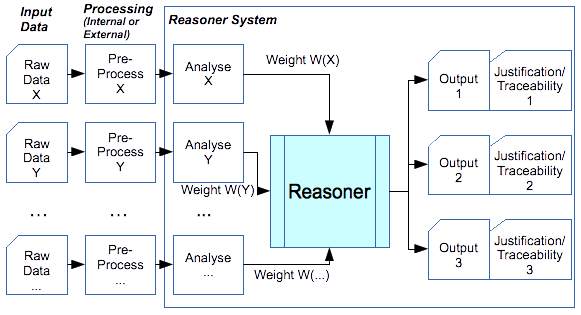
\includegraphics[scale=0.7]{sections/future/ReasonerDiagram}
\caption{Conceptual Diagram of Reasoning Component}
\label{fig-reasoning-component}
\end{figure}

\section{Visualisation and Developer Information}

Work towards an integrated application aimed at:

\begin{itemize}
\item Visualising software structures through utilisation of many different sources of information
\item Provide information to developers focused on change-impact e.g. for component A what other components are shown to be closely related and on what basis?
\end{itemize}

It is envisioned this will be an application (either standalone or more likely integrated within the D-UEA-ST framework) with which a developer can add multiple sources of information and may include the reasoning component (or at least output from the component). After an analysis has been automatically performed the developer will then be able to explore the software through an interface incorporating UML and textual representations, with more information on dependencies, relationships, and links to documentation provided.

\section{Requirements Traceability Reconstruction}

Using the above techniques investigate methods of rebuilding requirement links within the software (and feed this back into the process for example including requirement links within the visualiser).

\section{Work Plan}

The work plan is presented as a Gantt chart in figure \ref{fig-future-gantt}, including a one month contingency period and one month holiday in August 2014.

\begin{figure}[htb!]
\centering
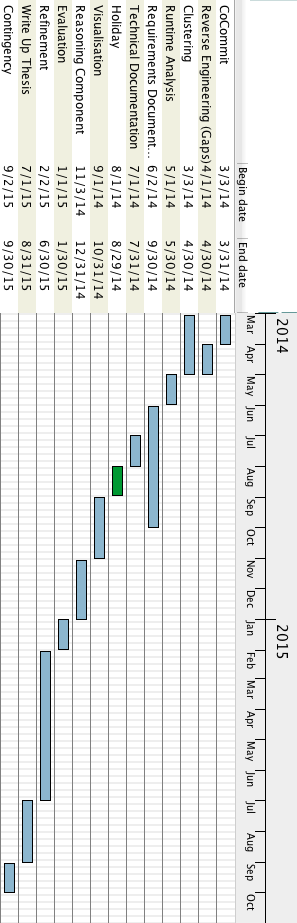
\includegraphics[scale=0.6]{sections/future/ProjectPlan-Rotate}
\caption{Project Gantt Chart}
\label{fig-future-gantt}
\end{figure}

\section{Possible Future Papers}

The following is a list of \textit{possible} potential papers from the future work. Whether they will be prepared (represent worthwhile findings) and the exact scope and size of the work will be decided as the project progresses. Potential targets are shown in \textit{( bracketed italics)} with the definitions of the conferences below.

\begin{itemize}
\item Commonalities Between Reverse Engineering and Repository Mining in Software Component Relationships \textit{(SANER, MSR)}
\item Building Complete Reverse Engineering Pictures from Multiple Partial or Failed Reverse Engineering Output \textit{(SANER, ECOOP, FASE, ACE)}
\item Augmenting Reverse Engineering with Additional Data Sources for Comprehensive Understanding \textit{(SANER, ECOOP, FASE, ACE)}
\item Visualising Software Relationships using Multiple Information Sources \textit{(FASE, ACE)}
\item Reasoning Software Structure in a Semi-Automated Fashion \textit{(FASE, ACE)}
\item Comparison of Structural Relationships Detected by Reverse Engineering, Repository Mining, and Runtime Analysis \textit{(SANER, MSR, FASE, ACE)}
\item Rebuilding Traceability Links from Multiple Sources of Information \textit{(FASE, ACE, ECOOP)}
\item Traceability Between Requirements Documentation, Technical Documentation, and Source Code Analysis \textit{(FASE, ACE, ECOOP)}
\end{itemize}

Targets for these potential papers would include:

\begin{itemize}
\item SANER: Merge of Working Conference on Reverence Engineering (WCRE) and European Conference on Software Maintenance and Re-engineering (CSMR)
\item ECOOP: European Conference on Object-Orientated Programming
\item FASE: Conference on the Fundamental Approaches to Software Engineering
\item ACE: ACE! Conference on Software Development
\item MSR: Conference on the Mining of Software Repositories
\end{itemize}